\documentclass[landscape, 11pt]{report}

% Packages
\usepackage[landscape]{geometry}
\usepackage{amsmath}
\usepackage{xcolor}
\usepackage[utf8]{inputenc}
\usepackage[russian]{babel}
\usepackage{geometry}
\usepackage{graphicx}

% Options
\graphicspath{ {../figures/} {./figures/}}
\geometry{left=2.5cm,right=2.5cm,top=2.5cm,bottom=2.5cm}
\setlength\parindent{0pt}

% Title
\title{
	
\includegraphics[scale=0.07]{logo}\\
	\vspace{0.5em}
	Языки программирования. Семантика и система типов\\
	\vspace{0.2em}
	\Large Теоретическое задание. Тема 3
}
\author{Бронников Егор}
\date{}


\begin{document}
	
	% Титул
	
	\maketitle
	
	\vspace{-0.5cm}
	\hrule
	\vspace{0.5cm}
	
	% Задание 1
	
	\textbf{Задание 1.} $(\lambda f . \, (f \, \{ \text{\color{purple}succ} \, \text{\color{blue}0}, \, \text{\color{purple}iszero} \, (f \, \{\text{\color{blue}0}, \, \text{\color{purple}false}\}).a \}).b) \, (\lambda t . \, \{a = t.1, \, b = t.2\})$
	
	\vspace{0.2cm}
	
	\textit{1. Дополнение пропущенных аннотаций.}
	
	$(\lambda f : \boldsymbol{Nat \times Bool \rightarrow \{a: Nat, \, b: Bool\}}. \, (f \, \{ \text{\color{purple}succ} \, \text{\color{blue}0}, \, \text{\color{purple}iszero} \, (f \, \{\text{\color{blue}0}, \, \text{\color{purple}false}\}).a \}).b) \, (\lambda t : \boldsymbol{Nat \times Bool}. \, \{a = t.1, \, b = t.2\}) : \boldsymbol{Bool}$
	
	\vspace{0.2cm}
	
	\textit{2. Дерево вывода типа.}
	
	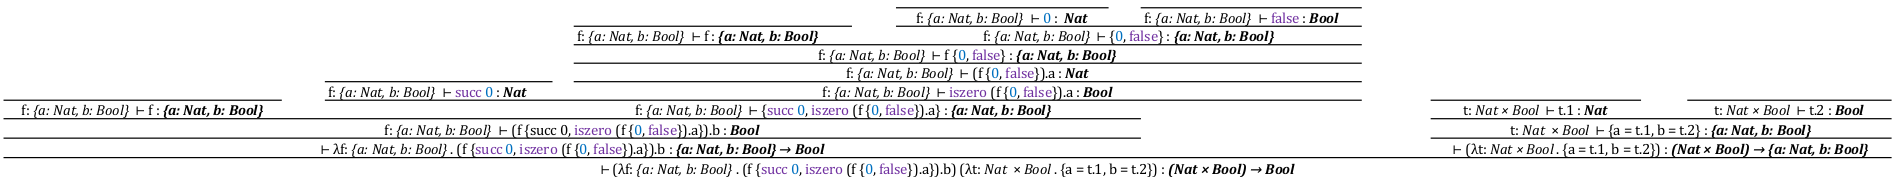
\includegraphics[scale=0.52]{task-1.png}

	\vspace{0.3cm}

	\small \textit{Примечание.} Рекомендуется изучить исходный Excel-документ \verb|source.xlsx|. \normalsize

	\vspace{0.2cm}
	\hrule
	\vspace{0.5cm}	
	
	% Задание 2
	
	\textbf{Задание 2.}

	\vspace{0.2cm}

	\textit{Условие.} В нетипизированном $\lambda$-исчисления, пары термов могут быть представлены при помощи кодировки Чёрча. Можно ли использовать это представление, чтобы представить пары как производную форму поверх простого типизированного $\lambda$-исчисления с логическими и арифметическими выражениями?
	
	\quad (a) Выпишите функцию раскрытия сокращений, соответствующих такому определению пар. Должны быть явно представлены раскрытия паро ($\{t_1, \, t_2\}$), проекции ($t.1$, $t.2$), и типа-произведения ($T_1 \times T_2$).
	
	\quad (b) Покажите, что функция раскрытия сокращений сохраняет вычисление и типизацию, если возможно. Иначе -- продемонстрируйте на контрпримере, почему сохранение вычисления или типизации невозможно.

	\vfill
	
	\footnotesize
	
	\begin{center}
		\textit{Смотреть продолжение на следующей странице.}
	\end{center}
	
	\normalsize

	\newpage

	\textit{Решение.}
	
	\vspace{0.2cm}

	\textit{a. Функция раскрытия сокращения.}
	
	\vspace{0.2cm}

	Пусть пара $\{t_1, \, t_2\}$ кодируется как $\lambda x \, y . \, x \, t_1 \, t_2$, тогда функция раскрытия сокращений будет иметь следующий вид:
	
	\begin{itemize}
		\item {Пара
			
			$pair \, t_1 \, t_2 = \lambda x \, y . \, x \, t_1 \, t_2$
		}
		
		\item {Первая проекция
			
			$first \, p = p \, (\lambda x . \, \lambda y . \, x) $
		}
		
		\item {Вторая проекция
			
			$second \, p = p \, (\lambda x . \, \lambda y . \, x)$
		}
	\end{itemize}
	
	Исходя из этого, раскрытие можно представить следующим образом:
	
	\begin{itemize}
		\item[] $\{t_1, \, t_2\} := pair \, t_1 \, t_2$
		\item[] $t.1 := first \, t$
		\item[] $t.2 := second \, t$
	\end{itemize}
	
	\textit{b. Сохранение вычисления и типизации}

	\begin{itemize}
		\item[] \textit{Сохранение вычисления.} Функция раскрытия сокращения должна преобразовывать термы таким образом, что результат вычисления преобразованного терма будет эквивалентен результату исходного вычисления. Так как кодировка Чёрча предоставляет точный механизм для представления пар и операций над ними, то вычисление будут сохраняться.
		\item[] \textit{Сохранение типизации.} При раскрытии сокращений типы термов должен быть сопоставимы с типами в исходном выражении. В типизированном $\lambda$-исчислении типы пар должны соответствовать ожидаемому обобщённому типу произведения. Если ${t : T}$ в исходной системе, то ${t' : T'}$ в преобразованной системе, таким образом, что $T$ соответствует $T'$. Однако в случае противоречия, когда типы не совпадают или не могут быть выведены, типизация термов не будет сохраняться.
	\end{itemize}

	\newpage
	
	Рассмотрим пары в типизированном $\lambda$-исчислении:
	
	\begin{center}
		$pair \, t_1 \, t_2 : T_1 \rightarrow T_2 \rightarrow (T_1 \rightarrow T_2 \rightarrow R) \rightarrow R$
	\end{center}

	В процессе раскрытия сокращений $pair \, t_1 \, t_2$ и применении функции $first$ или $second$, результатом будет $t_1$ или $t_2$. Это демонстрирует, что преобразованный терм сохраняет вычисление исходного терма.
	
	\vspace{0.2cm}
	
	Проблема сохранения типизации может возникать, потому что типизированное $\lambda$-исчисление накладывает ограничение на формы типов, которые может использовать в термах. Для пар $\{t_1, \, t_2\}$ тип каждого компонента $t_1$ и $t_2$ должен быть известен и типизирован отдельно, тогда как в нетипизированном $\lambda$-исчислении не существует данного ограничения.

	\vspace{0.5cm}
	
	\textit{Контрпример.}
	
	Пусть мы знаем, что $t_1 : T_1$ и $t_2 : T_2$. Используем $pair \, t_1 \, t_2$, тогда будет создан терм типа $\lambda x \, y . \, x \, t_1 \, t_2$, где $x$ и $y$ являются абстракциями переменных с типами $T_1$ и $T_2$, а $T_1$ и $T_2$ являются типами $t_1$ и $t_2$. Тогда тип данного терма будет неоднозначным, $T_1$ или $T_2$. Следовательно, это является нарушением правил типизации в контексте типизированного $\lambda$-исчисления.
	
	\vspace{0.5cm}
	
	\textit{Ответ.} Нельзя использовать кодировку Чёрча.

\end{document}
